\chapter{Discrete-time Systems}

\textbf{Discrete time} views values of variables as occurring at distinct, separate ``points in time'', or equivalently as being unchanged throughout each non-zero region of time (``time pe\-ri\-od'')---that is, \emph{time is viewed as a discrete variable} rather than as a continuous one. Thus a non-time variable jumps from one value to another as time moves from one time period to the next. This view of time corresponds to a digital clock that gives a fixed reading of 10:37 for a while, and then jumps to a new fixed reading of 10:38, etc. In this framework, each variable of interest is measured once at each time period. The number of measurements between any two time periods is finite. Measurements are typically made at sequential integer values of the variable ``time''~\cite{bib:discreteTimeSystems}.

A \textbf{discrete-time system} is a system that processes a given \emph{input sequence} $x[n]$ to generate an \emph{output sequence} $y[n]$ with certain characteristics derived from both the input sequence and the system. Typically, one has a single-input, single-output discrete-time system, whose general diagram is of the following kind,
\begin{center}
\begin{tikzpicture}

    \node                 (input)                                 {$x[n]$};
    \node[squarednode, thick, label=above:{\footnotesize{\emph{Discrete-time System}}}, minimum width=2cm]    (operation)     [right=of input]        {$\mathcal H(\cdot)$};
    \node                 (output)        [right=of operation]    {$y[n]$};

    \draw[->] (input.east) -- (operation.west);
    \draw[->] (operation.east) -- (output.west);
\end{tikzpicture}
\end{center}
Sure thing, the discrete-time system is characterized by an operator $\mathcal H(\cdot)$ that transforms the input sequence $x$ into another sequence $y$, the output. Resulting output will possess some characteristics that should be desirable and depend on the requirements.

We have already seen some examples of discrete-time systems. For instance, two of these were the \emph{modulator} and the \emph{adder} discrete-time systems, both $2$-input, $1$-output systems.
\begin{center}
    \begin{tikzpicture}
    \node [](A){$x[n]$};
    \node [draw, fill=black!15,circle,crossp, thick,minimum width=0.5 cm](B) at (1,0){};
    \node [](C) at(2,0){$z[n]$};
    \node [](D) at(1,-1){$y[n]$};
    \draw[->] (A) -- (B);
    \draw[->] (B) -- (C);
    \draw[->] (D) -- (B);
\end{tikzpicture}
\begin{tikzpicture}
    \node [](A) at (0,0){$x[n]$};
    \node [draw, fill=black!15,circle,plus,thick,minimum width=.5 cm](B) at (1,0){};
    \node [](C) at(2,0){$z[n]$};
    \node [](D) at(1,-1){$y[n]$};
    \draw[->] (A) -- (B);
    \draw[->] (B) -- (C);
    \draw[->] (D) -- (B);
\end{tikzpicture}
\end{center}
Other $1$-input, $1$-output discrete-time systems were the \emph{multiplier}, the \emph{unit delay} and the \emph{unit advance} we previously encountered in Section~\ref{sec:operationsOnSequences}.

In addition, multiple elementary operators may be combined together to form a much-more-complex discrete-time system. As an example, consider the one-input one-output discrete-time system in Figure~\ref{tikz:moreComplexDiscreteTimeSystem}.
\begin{figure*}
\begin{center}
    \begin{tikzpicture}
    \node [](input) at (0,0){$x[n]$};
    \node [draw, dot](B) at (1,0){};
    \node [draw, boxfilter](C) at (2,0){$z^{-1}$};
    \node [draw, fill=black!5,circle,plus,thick,minimum width=.5 cm](adder) at (4,-3){};
    \node [draw, dot, label=above:{$x[n-1]$}](D) at (3,0){};
    \node [draw, boxfilter](E) at (4,0){$z^{-1}$};
    \node [draw, dot, label=above:{$x[n-2]$}](F) at (5,0){};
    \node [draw, boxfilter](G) at (6,0){$z^{-1}$};
    \node [draw, dot, label=above:{$x[n-3]$}] (H) at (7,0){};
    \node [draw, multiplierdownwards, label=north east:{$\alpha_1$}](alpha1) at (1,-1){};
    \node [draw, multiplierdownwards, label=north east:{$\alpha_2$}](alpha2) at (3,-1){};
    \node [draw, multiplierdownwards, label=north east:{$\alpha_3$}](alpha3) at (5,-1){};
    \node [draw, multiplierdownwards, label=north east:{$\alpha_4$}](alpha4) at (7,-1){};
    \node [](output) at (4,-4){$y[n]$};

    \draw[thick] (input) -- (B);
    \draw[-stealth, thick] (B) -- (C);
    \draw[thick] (C) -- (D);
    \draw[-stealth, thick] (D) -- (E);
    \draw[thick] (E) -- (F);
    \draw[-stealth, thick] (F) -- (G);
    \draw[-stealth, thick] (G) -- (H) -- (alpha4);
    \draw[-stealth, thick] (B) -- (alpha1);
    \draw[-stealth, thick] (D) -- (alpha2);
    \draw[-stealth, thick] (F) -- (alpha3);
    \draw[-stealth, thick] (alpha1) |- (adder);
    \draw[-stealth, thick] (alpha2) -- (3,-2) -- (adder);
    \draw[-stealth, thick] (alpha3) -- (5,-2) -- (adder);
    \draw[-stealth, thick] (alpha4) |- (adder);
    \draw[-stealth, thick] (adder) -- (output);

\end{tikzpicture}\caption{A one-input, one-output discrete-time system that shows concatenation of multiple elementary operators to form a more complex graph and a more convoluted input--output relationship.} \label{tikz:moreComplexDiscreteTimeSystem}
\end{center}
\end{figure*}

\section{Fundamental Discrete-time Systems}

\subsection{Accumulator}

The first fundamental discrete-time system we will meet is the \textbf{accumulator} system. An accumulator is led by the following relationship
\begin{align}
    y[n] &= \sum_{i=-\infty}^{n} x[i] \\
         &= \sum_{i=-\infty}^{n-1} x[i] + x[n]\\
         &= y[n-1] + x[n].\label{eqn:accumulatorEquation}
\end{align}
which establishes that the output $y[n]$ at the time instant $n$ is the sum of two terms, the first one being the input at the time instant $n$, $x[n]$, and the second one being the previous output $y[n-1]$ at the previous time instant $n-1$. The latter addendum is the sum of all previous input sample values, from the beginning of the signal to the previous time instant---that is, from sample $-\infty$ to sample $n-1$.

An accumulator, as its name suggests, \emph{cumulatively adds} all input sample values from the beginning of the signal history up to the current time instant $n$. This behavior is indeed evident by looking at the terms in the sides of Equation~\ref{eqn:accumulatorEquation}.

Any accumulator could be split into two terms, a first being a constant, and the second one capable of describing a \emph{causal} input sequence. In truth,
\begin{align}
    y[n] &= \sum_{i=-\infty}^{n} x[i] \\
         &= \sum_{i=-\infty}^{-1} x[i] + \sum_{i=0}^{n}x[i]\\
         &= y[-1] + \sum_{i=0}^n x[n].\label{eqn:accumulatorCausalEquation}
\end{align}
where the first term $y[-1]$ is said to be \emph{initial condition}, while the second term is fit to describe a \emph{causal} input sequence, as it is a sum starting from time instant $0$. Basically, this means that \emph{any accumulator can be described with a causal input sequence and with its initial conditions}, as \ref{eqn:accumulatorCausalEquation} suggests. This property reveals to be of paramount importance when describing accumulators in general, especially if one wants to build a discrete-time system that only takes in account causal input signals, starting from time interval $0$ and going on.

\subsection{$M$-point Moving-Average System}

The \textbf{$M$-point Moving Average System} is a discrete-time system described by the input--output relationship
\begin{equation}\label{eqn:mPointMovingAverageEquation}
    y[n] = \frac 1 M \sum_{k=0}^{M-1} x[n-k].
\end{equation}
The $M$-point attribute is related to the fact that---starting from time instant $0$---exactly $M$ points are averaged together, while ``moving'' stands for the fact that the value of the system can be interpreted as a constantly-moving average between points, since the output value will vary as new input samples are added to the sum.

In most applications, the input data $x[n]$ is a bounded sequence; therefore, the $M$-point average $y[n]$ is a bounded sequence as well. Doubtlessly, if there is no bias in the measurements, an improved estimate of the noisy data is obtained by simply increasing the value of $M$.

A direct implementation of the moving average discrete-time system requires $M-1$ additions, a single division and the storage of $M-1$ past input data samples. As we will see later on, this is far from the most efficient solution.

The $M$-point moving average system can be rewritten as follows,
\begin{align*}
    y[n] &= \frac 1 M \left(\sum_{l=0}^{M-1}x[n-l]\right) \\
         &= \frac 1 M \left(\sum_{l=1}^{M-1}x[n-l] + x[n]\right)\\
         &= \frac 1 M \left(\sum_{l=1}^{M-1}x[n-l] + x[n] + x[n - M] - x[n - M]\right)\\
         &= \frac 1 M \left(\sum_{l=1}^{M}x[n-l] + x[n] - x[n - M]\right)\\
         &= \frac 1 M \left(\sum_{l=0}^{M-1}x[n-1-l] + x[n] - x[n - M]\right)\\
         &= \frac 1 M \left(\sum_{l=0}^{M-1}x[n-l-1]\right) + \frac 1 M \left(x[n] - x[n - M]\right)\\
    y[n] &= y[n-1] + \frac 1 M \left(x[n] - x[n - M]\right).
\end{align*}

We have just witnessed how the computation of the modified $M$-point moving average system---rearranging the \emph{recursive equation}---requires \emph{only $2$ additions and $1$ division}, in contrast with the previous case where a number of operations dependent on the number of samples $M$ was necessary. An apparently unvalicable computation limit had been removed just by cleverly rearranging the equation of the system involved. Later on, we will see other cases in which this is true and very desirable.

An application for the $M$-point moving average system is the following one: let a sequence $x[n]$ be the sum of two sequences, the first one being a sequence $s[n]$ obtained from a signal which is inevitably corrupted by a noise $d[n]$, hence \[x[n] = s[n] + d[n].\] Usually, the noise is a small part of the signal; still, the original signal is somehow corrupted by the presence of the noise in such a way that sometimes noise reduction techniques are auspicable. A common §FIXME

\subsection{Exponentially Weighted Running Average Filter}

The \textbf{Exponentially Weighted Running Average Filter} is a kind of filter expressed by the relationship
\begin{equation}\label{eqn:exponentiallyWeightedRunningAverageFilterEquation}
    y[n] = \alpha y[n-1] + x[n], 0 < \alpha < 1.
\end{equation}
Since $0 < \alpha < 1$, the exponentially weighted average filter places a lot more emphasis on \emph{current} data samples than \emph{past} data samples, as all the previous preocessed data is multiplied by a constant factor which is smaller than $1$. If $x[n]\equiv 0$ at some time interval and for all future samples, the output $y[n]$ is condemned to decay and collapse to $0$ at a speed that substantially depends on the value of $\alpha$.

In fact, this is soon shown by just substituting recursively the definition with itself,
\begin{align*}
    y[n] &= \alpha y[n-1] + x[n]\\
         &= \alpha(\alpha y[n-2] + x[n-1]) + x[n]\\
         &= \alpha^2(\alpha y[n-3] + x[n-2]) + \alpha x[n-1] + x[n]\\
         &= \alpha^3y[n-3] + \alpha^2 x[n-2] + \alpha x[n-1] + x[n]
\end{align*}
where it is immediately clear that the terms with $\alpha$ of higher order tend to be smaller as the order increases.

Computation of the running average filter only requires a single addition and a single multiplication; still, it requires storage of the previously-run average value. As a bonus, it does not require the storage of the full-chain of past data samples.

\subsection{Median Filter}

The \textbf{median filter} of a set of $2K+1$ numbers is the number such that $K$ numbers from the set possess values that are greater than this number, while the other $K$ numbers have lower values. The median can be determined by performing a rank-ordering of the numbers in the set by their values, and ultimately choosing the number at the middle of the just produced sequence. In short, the median filter computes \emph{the median in the window}.

A median filter is usually implemented by a sliding window of \emph{odd} length, over the entire input sequence $x[n]$, moving the window from left to right one sample at a time. The output $y[n]$ at instant $n$ is the median value of the samples inside the sliding window that is currently centered at $n$.

Median filters are very good at removing both \emph{shot noise} (impulse-like noise) and \emph{random noise}, either of additive or substitutive kind---especially in the case of sudden, large errors in the corrupted signal. For this reason, median filters are applied to smooth a shot-noise-corrupted signal.


\section{Linear interpolation}

The \textbf{linear interpolation} is a technique that is adopted to estimate sample values between pairs of adjacent sample values of a discrete-time sequence. To perform that, additional samples are added in between two adjacent values (upsampling), and then a further interpolation technique is adopted by means of \emph{linearly connecting the values}.

The linear interpolation can be expressed as in Figure~\ref{tikz:linearInterpolationFactorFour}

\begin{figure*}[ht]
    \begin{center}
        \begin{tikzpicture}[scale=1.2]
            %\node[above,font=\large\bfseries] at (0,3.5) {Unit sample se\-quen\-ce};
            \draw[->] (-0.5,0) -- (6.5,0) node[anchor=north west] {$t$};
            \draw[] (0,0) -- (0,1);
            \draw[] (2,0) -- (2,-.7);
            \draw[] (4,0) -- (4,2);
            \draw[] (6,0) -- (6,.4);

        \foreach \x in {0,1,2,3}
            \draw (2*\x cm,1pt) -- (2*\x cm,-1pt) node[inner sep=0pt, anchor=north,label=south east:{$\x$}] {};

            \node at (0,3) {$(a) \mbox { } x[n]$};
            \node [draw,inner sep=1pt, circle, thick](A) at (0,1){};
            \node [draw,inner sep=1pt, circle, thick](B) at (2,-0.7){};
            \node [draw,inner sep=1pt, circle, thick](C) at (4,2){};
            \node [draw,inner sep=1pt, circle, thick](D) at (6,.4){};
        \end{tikzpicture}
        \\
        \vspace*{1cm}
        \begin{tikzpicture}[scale=1.2]
            %\node[above,font=\large\bfseries] at (0,3.5) {Unit sample se\-quen\-ce};
            \draw[->] (-0.5,0) -- (6.5,0) node[anchor=north west] {$t$};
            \draw[] (0,0) -- (0,1);
            \draw[] (2,0) -- (2,-.7);
            \draw[] (4,0) -- (4,2);
            \draw[] (6,0) -- (6,.4);

        \foreach \x in {0,1,2,...,12}
            \draw (0.5*\x cm,1pt) -- (0.5*\x cm,-1pt) node[inner sep=0pt, anchor=north,label=south east:{$\x$}] {};

            \node at (0,3) {$(b) \mbox { } x_u[n]$};
            \node [draw,inner sep=1pt, circle, thick](A) at (0,1){};
            \node [draw,inner sep=1pt, circle, thick](B) at (2,-0.7){};
            \node [draw,inner sep=1pt, circle, thick](C) at (4,2){};
            \node [draw,inner sep=1pt, circle, thick](D) at (6,.4){};
            \node [draw,inner sep=1pt, circle, thick](Ab) at (.5,0){};
            \node [draw,inner sep=1pt, circle, thick](Ac) at (1,0){};
            \node [draw,inner sep=1pt, circle, thick](Ad) at (1.5,0){};
            \node [draw,inner sep=1pt, circle, thick](Bb) at (2.5,0){};
            \node [draw,inner sep=1pt, circle, thick](Bc) at (3,0){};
            \node [draw,inner sep=1pt, circle, thick](Bd) at (3.5,0){};
            \node [draw,inner sep=1pt, circle, thick](Cb) at (4.5,0){};
            \node [draw,inner sep=1pt, circle, thick](Cc) at (5,0){};
            \node [draw,inner sep=1pt, circle, thick](Cd) at (5.5,0){};
        \end{tikzpicture}
        \\
        \vspace*{1cm}
        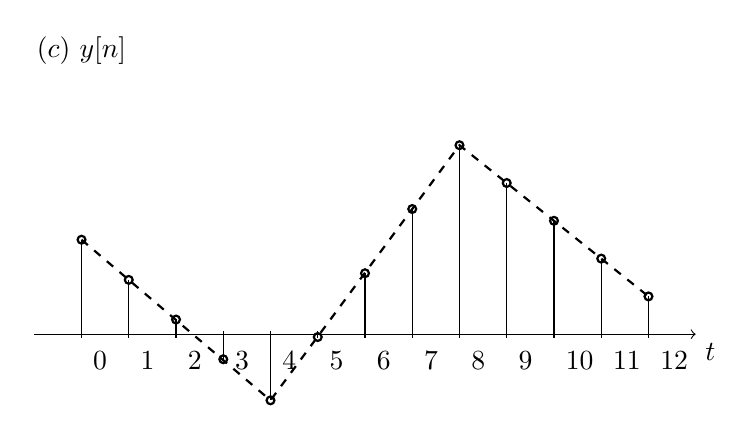
\begin{tikzpicture}[scale=1.2]
            %\node[above,font=\large\bfseries] at (0,3.5) {Unit sample se\-quen\-ce};
            \draw[->] (-0.5,0) -- (6.5,0) node[anchor=north west] {$t$};
            \draw[] (0,0) -- (0,1);
            \draw[] (2,0) -- (2,-.7);
            \draw[] (4,0) -- (4,2);
            \draw[] (6,0) -- (6,.4);

        \foreach \x in {0,1,2,...,12}
            \draw (0.5*\x cm,1pt) -- (0.5*\x cm,-1pt) node[inner sep=0pt, anchor=north,label=south east:{$\x$}] {};

            \node at (0,3) {$(c) \mbox { } y[n]$};
            \node [draw,inner sep=1pt, circle, thick](A) at (0,1){};
            \node [draw,inner sep=1pt, circle, thick](B) at (2,-.7){};
            \node [draw,inner sep=1pt, circle, thick](C) at (4,2){};
            \node [draw,inner sep=1pt, circle, thick](D) at (6,.4){};
            \node [draw,inner sep=1pt, circle, thick](Ab) at (.5,.575){};
            \draw[] (.5,0) -- (.5,.575);
            \node [draw,inner sep=1pt, circle, thick](Ac) at (1,0.155){};
            \draw[] (1,0) -- (1,.155);
            \node [draw,inner sep=1pt, circle, thick](Ad) at (1.5,-0.265){};
            \draw[] (1.5,0) -- (1.5,-.265);
            \node [draw,inner sep=1pt, circle, thick](Bb) at (2.5,-.03){};
            \node [draw,inner sep=1pt, circle, thick](Bc) at (3,.645){};
            \draw[] (3,0) -- (3,.645);
            \node [draw,inner sep=1pt, circle, thick](Bd) at (3.5,1.325){};
            \draw[] (3.5,0) -- (3.5,1.325);
            \node [draw,inner sep=1pt, circle, thick](Cb) at (4.5,1.6){};
            \draw[] (4.5,0) -- (4.5,1.6);
            \node [draw,inner sep=1pt, circle, thick](Cc) at (5,1.20){};
            \draw[] (5,0) -- (5,1.20);
            \node [draw,inner sep=1pt, circle, thick](Cd) at (5.5,0.8){};
            \draw[] (5.5,0) -- (5.5,0.8);

            \draw[thick, dashed] plot coordinates {(0,1) (2,-.7) (4,2) (6,.4)};
        \end{tikzpicture}
    \end{center}\caption{Interpolation of a signal $x[n]$ with factor of $4$. From top to bottom: $(a)$ original signal $x[n]$, $(b)$ upsampled version $x_u[n]$ and $(c)$ interpolated output sequence $y[n]$.}\label{tikz:linearInterpolationFactorFour}
\end{figure*}

Linear interpolation can never produce a correct output sequence. This is because---if the real signal were the dashed line in \ref{tikz:linearInterpolationFactorFour}---a signal whose derivative is infinite at some points would require \emph{infinite} band, therefore an infinite sampling rate would be necessary.

Mathematically, interpolation having factors of $2$ and $3$ might be expressed, respectively for sequences $y_2[n]$ and $y_3[n]$, as follows,
\begin{align*}
    y_2[n] &= x_u[n] + \frac 1 2(x_u[n-1] + x_u[n+1]);\\
    y_3[n] &= x_u[n] + \frac 1 3(x_u[n-2] + x_u[n+2])\\
           &+ \frac 2 3(x_u[n-1] + x_u[n+1]),
\end{align*}
with the \emph{low-frequency gain} equal to $\mbox{DCGain} = L$. Notice that a formally correct solution would require much more complex operators.

\clearpage

\section{Classification of Discrete-time Systems}

\subsection{Linear Discrete-time Systems}

A \textbf{Linear Discrete-time System} is any special kind of discrete-time system such that, if $y_1$ is the output of the input $x_1$ and $y_2$ is the output from the input $x_2$, then f or an input that is the combination of the two inputs $x_1$ and $x_2$
\begin{equation*}
    x[n] = \alpha x_1[n] + \beta x_2[n],
\end{equation*}
the output is given by the \emph{superposition} of outputs
\begin{equation}\label{eqn:linearDiscreteTimeSystem}
    y[n] = \alpha y_1[n] + \beta y_2[n].
\end{equation}
The above property is fundamental for any linear discrete-time system, and must hold for any arbitrary constant $\alpha$ and $\beta$, for all possible combination of input sequences $x_1[n]$ and $x_2[n]$, and it is called the \textbf{superposition principle}.

Discrete-time Systems that follow the superposition principle and are thus linear are all the accumulators. Indeed, given an accumulator output to two inputs,
\begin{align*}
    y_1[n] &= \sum_{l=-\infty}^n x_1[l], \\
    y_2[n] &= \sum_{l=-\infty}^n x_2[l],
\end{align*}
for an input supercomposed of $x[n] = \alpha x_1[n] + \beta x_2[n]$ the corresponding output of the accumulator is
\begin{align*}
    y[n] &= \sum_{l=-\infty}^n (\alpha x_1[l] + \beta x_2[l]) \\
         &= \alpha\sum_{l=-\infty}^n x_1[l] + \beta\sum_{l=-\infty}^n x_2[l]
\end{align*}
which indeed shows that any accumulator is a \emph{linear} discrete-time system.

Moreover, since they follow the superposition principle, a property analogous of Equation~\ref{eqn:accumulatorCausalEquation} holds---that is, given
\begin{align*}
    y_1[n] &= y_1[-1] + \sum_{l=0}^n x_1[l], \\
    y_2[n] &= y_2[-1] + \sum_{l=0}^n x_2[l],
\end{align*}
by the superposition principle one gets
\begin{align*}
    \alpha y_1[n] + \beta y_2[n]  &= \alpha ( y_1[-1] + \sum_{l=0}^n x_1[l]) + \beta ( y_2[-1] + \sum_{l=0}^n x_2[l])\\
                                  &= (\alpha y_1[-1] + \beta y_2[-1]) + (\alpha\sum_{l=0}^n x_1[l] + \beta\sum_{l=0}^n x_2[l]),
\end{align*}
and for this reason $y[n] = \alpha y_1[n] + \beta y_2[n]$ if and only if
\begin{equation}\label{eqn:accumulatorInitialCondition}
    y[-1] = \alpha y_1[-1] + \beta y_2[-1],
\end{equation}
a severe equation that establishes a precise condition under which the initial condition must undergo. For any accumulator with a causal input to be \emph{linear} the condition expressed in Equation~\ref{eqn:accumulatorInitialCondition} must hold for all initial conditions $y[-1]$, $y_1[-1]$, $y_2[-1]$ and for all constants $\alpha$ and $\beta$. Still, the condition can never be satisfied---unless the accumulator is \emph{initially at rest}, with zero initial condition. That practically means having
\[
    y[-1] = \alpha y_1[-1] + \beta y_2[-1] \equiv 0.
\]

\subsection{Nonlinear Discrete-time Systems}

A \textbf{Nonlinear Discrete-time System} is any system that does not comply with the superposition principle. To name one, the median filter is a nonlinear system. To prove that, consider outputs for the following inputs (median filter with window size of $3$),
\begin{align*}
    \{x_1[n]\} = \{3,4,5\}, 0 \leq n \leq 2 &\longrightarrow \{y_1[n]\}=\{3,4,4\}, 0 \leq n \leq 2,\\
    \{x_2[n]\} = \{2,-1,-1\}, 0 \leq n \leq 2 &\longrightarrow \{y_2[n]\}=\{0,-1,-1\}, 0 \leq n \leq 2,\\
    \{x[n]\} = \{x_1[n] + x_2[n]\} &\longrightarrow \{y[n]\}=\{3,4,3\}
\end{align*}
but
\[\{y_1[n] + y_2[n]\} = \{3, 3, 3\}\]
which is different from $\{y[n]\}$; hence, the median filter is a nonlinear discrete-time system, for which the superposition principle doesn't apply.

Another example of nonlinear discrete-time system is the second form of the accumulator with non-zero initial condition, for which the term $y[-1] \neq 0$.

\subsection{Shift-Invariant Systems}

Any \textbf{Shift-Invariant System} is a system for which if the response to an input $x_1[n]$ is $y_1[n]$, then the response to an input \[x[n] = x_1[n-n_0]\] where $n_0 \in \Z$ is the translation of the output as well, that is \[y[n] = y_1[n-n_0].\] The above property is called the \emph{time-invariance property}.

The above relationship must hold for any arbitrary input and its corresponding input. This means that by simply shifting the input sequence one obtains an output sequence which is shifted as well, by the same quantity as the shift of the input sequence.

Time-invariance property ensures that---for a specified input---the output is independent of the time the input is being applied.

As an example of a \textbf{non}-complying system, consider an up-sampler with an input-output relationship given by
\[
	x_u[n] =
	\left\{
		\begin{array}{ll}
			x[n/L] 	& n=0,\pm L, \pm 2L, \dots \\
			0 	& otherwise
		\end{array}
	\right.
\]

For a new input $\hat x[n] = x[n-n_0], n_0 \in \Z$, one obtains the output
\begin{align*}
    \hat x_u[n] &=
	\left\{
		\begin{array}{ll}
			\hat x[n/L] 	& n=0,\pm L, \pm 2L, \dots \\
			0 	& otherwise
		\end{array}
	\right.\\
                &=
    \left\{
		\begin{array}{ll}
            x[\frac{n-Ln_0}{L}] 	& n=0,\pm L, \pm 2L, \dots \\
			0 	& otherwise
		\end{array}
	\right.
\end{align*}
which is indeed \emph{different} from what one obtains by applying the definition straightforwardly, that is
\begin{align*}
    \hat x_u[n-n_0] &=
	\left\{
		\begin{array}{ll}
            \hat x[\frac{n-n_0}{L}] 	& n=n_0,\pm L,n_0 \pm 2L, \dots \\
			0 	& otherwise
		\end{array}
	\right.\\
                    &\neq \hat x_u[n]
\end{align*}
as time instant on the numerator is shifted by $n_0$ and not by $Ln_0$. When a discrete-time system is not shift-invariant, it is said to be a \emph{time-varying system}.

\subsection{Linear Time-Invariant Systems}\label{sec:ltiSystems}

A much important class of discrete-time systems is the class of the \textbf{Linear Time-Invariant (LTI) Systems}. An LTI system is any system that it is both linear and shift-invariant---that is a system satisfying both the superposition principle and the time-invariance property. LTI systems are mathematically easy to deal with, to analyze and to characterize. As a consequence, they are very easy to design compared to other ``harder'' signals. Indeed, highly useful signal processing algorithms have been developed by means of this class of systems over the last several decades.

\subsection{Causal Systems}

In a \textbf{Causal System}, the $n_0$-th output sample $y[n_0]$ depends only on input samples $x[n]$ for $n\leq n_0$; this means that the output depends only on the input from time instants \emph{before} the current one ($n_0$), and does not depend on future input samples $n \geq n_0$.

Let $y_1[n]$ and $y_2[n]$ be the responses of a causal, discrete-time system to the inputs $x_1[n]$ and $x_2[n]$, respectively. Then, \begin{equation}\label{eqn:causalDiscreteTimeSystemsEquation}x_1[n] = x_2[n], n < N \Longrightarrow y_1[n] = y_2[n], n < N.\end{equation}
Equation~\ref{eqn:causalDiscreteTimeSystemsEquation} implies that for a causal system all changes in output samples never precede changes in the input samples.
Examples of causal systems are the signals $y_{c,1}$, $y_{c,2}$, and $y_{c,3}$,
\begin{align*}
    y_{c,1}[n] &= \alpha_1 x[n] + \alpha_2 x[n-1]\\
               &+ \alpha_3 x[n-2] + \alpha_4 x[n-3]\\
    y_{c,2}[n] &= \beta_0 x[n] + \beta_1 x[n-1] + \beta_2 x[n-2]\\
               &+ \alpha_1 y[n-1] + \alpha_2 y[n-2]\\
    y_{c,3}[n] &= y[n-1] + x[n],
\end{align*}
while a noncausal system is, for example, the sequence of a linear interpolation $y_{nc}[n]$,
\begin{align*}
    y_{nc}[n] &= x_u[n] + \frac 1 3(x_u[n-2] + x_u[n+2])\\
           &+ \frac 2 3(x_u[n-1] + x_u[n+1]).
\end{align*}

Any noncausal system can still be implemented as a causal system; this is done by delaying the output by an appropriate number of samples. For instance, a causal implementation of the factor-of-two interpolator---an otherwise noncausal system---is given by
\begin{equation}\label{eqn:causalLinearInterpolationFactorTwo}
    y[n] = x_u[n-1] + \frac 1 2(x_u[n-2] + x_u[n]).
\end{equation}
The trick here is to delay of a single unit the entire filter, so that the time instant $n+1$ is simply shifted to $n$ in order to produce a causal system. Since a noncausal system has a finite $N$ such that $n+N > n$, it will always be possible to time-delay of $N$ the entire noncausal system so that it fits the property of causality so that $n + N$ becomes $n$.

\subsection{Stable Systems}\label{sec:BIBOStableSystems}

Since there are various definition of stability, one has to first choose an appropriate one before giving the definition of stable systems. We consider the \textbf{Bounded-Input, Bounded-Output (BIBO) stability}.

If $y[n]$ is the response to an input $x[n]$, and if \[|x[n]| \leq B_x, \forall n,\] then the system is \emph{BIBO stable} if \[|y[n]| \leq B_y,\forall n.\]

An example of a BIBO stable system is soon provided. Consider an $M$-point moving average filter as in Equation~\ref{eqn:mPointMovingAverageEquation},
\[
    y[n] = \frac 1 M \sum_{k=0}^{M-1} x[n-k].
\]
Against a bounded input $|x[n]| \leq B_x < \infty$ one obtains
\begin{align*}
    |y[n]| &= \left| \frac 1 M \sum_{k=0}^{M-1} x[n-k]\right|\\
           &= \frac 1 M \sum_{k=0}^{M-1} \left| x[n-k]\right|\\
           &= \frac 1 M (MB_x) = B_x.
\end{align*}

BIBO stable systems are indeed important, as they are all systems for which---provided the input is known to be bounded---the output will be necessarily bounded.

\subsection{Passive and Lossless Systems}

Discrete-time systems are defined to be \textbf{passive} if, for every finite-energy input $x[n]$ the output $y[n]$ has---at most---the very same energy, that is
\begin{equation}\label{eqn:passiveSystemsDefinition}
    \mathcal E_y = \sum_{n=-\infty}^{\infty} | y[n] |^2
    \leq \mathcal E_x = \sum_{n=-\infty}^{\infty} | x[n] |^2 < \infty
\end{equation}
Any passive system \emph{can never increase the energy} of the input sequence.

A particular case of discrete-time systems are the \textbf{lossless} systems, for which the output $y[n]$ possesses the very same energy---there is no energy loss through the system. This means that for a lossless system it goes that
\begin{equation}\label{eqn:losslessSystemsDefinition}
    \mathcal E_y = \sum_{n=-\infty}^{\infty} | y[n] |^2
    = \mathcal E_x = \sum_{n=-\infty}^{\infty} | x[n] |^2 < \infty
\end{equation}

Suppose to have the following discrete-time system defined by the relationship
\[
    y[n] = \alpha x[n-N], N\in\N.
\]
The output energy for such a system is given by
\[
    \sum_{n=-\infty}^{\infty} |y[n]|^2 = |\alpha|^2 \sum_{n=-\infty}^{\infty}|x[n]|^2,
\]
and it depends on the choice of the coefficient $\alpha$, as it is either a passive system if $|\alpha| < 1$, or a lossless system in the case of $|\alpha| = 1$. Of course, it is neither passive nor lossless if $|\alpha| > 1$.

\subsection{Impulse and Step Response of a Discrete-time System}

The \textbf{unit sample response} or the \textbf{impulse response} of a discrete-time system is the response of such system to a unit sample sequence $\{\delta[n]\}$ and it is usually denoted as $\{h[n]\}$.

Correspondingly, the \textbf{unit step response} or the \textbf{step response} of a discrete-time system is the response of such system to a unit step sequence $\{\mu[n]\}$ and it is commonly denoted by $\{s[n]\}$.

Both responses play a crucial role when studying the properties of discrete-time systems.

Suppose one has the following system
\begin{align*}
    y[n] &= \alpha_1 x[n] + \alpha_2 x[n-1]\\
               &+ \alpha_3 x[n-2] + \alpha_4 x[n-3];
\end{align*}
the impulse response is soon obtained by setting $x[n] = \delta[n]$ as input sequence and evaluating the result:
\begin{align*}
    h[n] &= \alpha_1 \delta[n] + \alpha_2 \delta[n-1]\\
               &+ \alpha_3 \delta[n-2] + \alpha_4 \delta[n-3].
\end{align*}

Therefore, the impulse response is a finite-length \emph{sequence} of length $4$, which is given by
\[
    \{h[n]\} = \begin{Bmatrix}\underset{\uparrow}{\alpha_1} & \alpha_2 & \alpha_3 & \alpha_4\end{Bmatrix}
\]

The example shows that---for a specific class of sequences---the impulse response happens to be similar to the sequence of the coefficients of the relationship, a rule that is not true in general.

Let's now study the impulse response of the discrete-time accumulator. One has
\[
    y[n] = \sum_{i=-\infty}^{n} x[i];
\]
by substituting with the impulse sequence one gets
\[
    h[n] = \sum_{i=-\infty}^{n} \delta[l] = \mu[n].
\]

Since what an accumulator does, roughly speaking, is to ``collect and sum up all the values of a sequence up to time instant $n$'', its impulse response will be $0$ up to the origin, after which the value of $1$ will be collected. Undoubtedly, this sounds like performing an ``integration'' operation, although there are some substantial differences involved.§FIXME

The impulse response $h[n]$ of the factor-of-two interpolator
\[
    y[n] = x_u[n] + \frac 1 2(x_u[n-1] + x_u[n+1])
\]
is obtained, in the same manner, by setting $x_u[n]=\delta[n]$ and is ultimately
\[
    h[n] = \delta[n] + \frac 1 2(\delta[n-1] + \delta[n+1])
\]
which yields the finite-length sequence having length $3$
\[
    \{h[n]\} = \{0.5, \underset{\uparrow}{1}, 0.5\}.
\]

\section{Time-Domain Characterization of LTI Discrete-time Systems}

\subsection{The Convolution Sum}

LTI discrete-time system possess peculiar characteristic for their input--output relationship. A consequence of the linear time-invariance property combination is that any LTI discrete-time system is completely characterized by its own impulse response $h[n]$. Since the impulse response is subject to both superposition principle and it is invariant to shifts of any entity, it suffices to know the impulse response to compute the output of the system for any arbitrary input sequence $x[n]$.

In fact, let $h[n]$ denote the impulse response of an LTI discrete-time system. For instance, let an input be
\[
    x[n] = 0.5\delta[n+2] + 1.5\delta[n-1] - \delta[n-2] + 0.75\delta[n-5];
\]
in order to compute the output $y[n]$ one has to compute its outputs for each addendum separately, and finally adding the individual outputs (superposition principle). As the system is also time-invariant, the rule that governs the input--output relation is the following one,
\begin{equation}\label{eqn:impulseResponseLTI}
    \overset{input}{\delta[n-k]} \longrightarrow \overset{output}{h[n-k]}.
\end{equation}

Under that rule, it's easy to determine the output relative to each and every addendum, as they are
\begin{align*}
    \overset{input}{0.5\delta[n+2]} & \longrightarrow \overset{output}{0.5h[n+2]},\\
    1.5\delta[n-1] & \longrightarrow 1.5h[n-1],\\
    -\delta[n-2] & \longrightarrow -h[n-2],\\
    0.75\delta[n-5] & \longrightarrow 0.75h[n-5];
\end{align*}
in the end---thanks to the superposition principle---one gets
\[
    y[n] = 0.5h[n+2] + 1.5h[n-1] - h[n-2] + 0.75h[n-5].
\]

This example highlights the fact that, both superposition principle and shift-invariance prove useful to immediately compute the impulse response of any LTI system. Indeed, since an arbitrary input $x[n]$ can be rewritten as a sum of (many) unit impulses
\begin{equation}\label{eqn:inputAsSumOfImpulses}
    x[n] = \sum_{k=-\infty}^\infty x[k] \delta[n-k],
\end{equation}
the response of an LTI system to an input of such form will be
\begin{equation}\label{eqn:impulseResponseLTIArbitrary}
    y[n] = \sum_{k=-\infty}^\infty x[k] h[n-k],
\end{equation}
because of input--output relationship expressed by~\ref{eqn:impulseResponseLTI}. And after rewriting it, one obtains a completely equivalent formulation
\begin{equation}\label{eqn:impulseResponseLTIArbitraryAlternate}
    y[n] = \sum_{k=-\infty}^\infty x[n-k] h[k].
\end{equation}

Equations~\ref{eqn:impulseResponseLTIArbitrary}~and~\ref{eqn:impulseResponseLTIArbitraryAlternate} both describe the same operation known as the \textbf{convolution sum} of the sequences $x[n]$ and $h[n]$. The operation is so important that a specific operator has been adopted,
\begin{equation}\label{eqn:convolutionSum}
    y[n] = x[n] \circledast h[n].
\end{equation}

The properties of the convolution sum are the following ones\footnote{An important remark on this is that the following properties hold only for \emph{infinite-precision} and \emph{infinite-range} representations, as truncated ones might suffer from §FIXME}:
\begin{itemize}
    \item the convolution is \emph{commutative},\[ g[n] \circledast h[n] = h[n] \circledast g[n];\]
    \item the convolution is \emph{associative},\[ (g[n] \circledast h[n]) \circledast k[n] = g[n] \circledast (h[n] \circledast k[n]);\]
    \item the convolution is \emph{distributive},\[ g[n] \circledast (h[n] + k[n]) = g[n] \circledast h[n] + g[n] \circledast k[n].\]
\end{itemize}

Any convolution sum can be interpreted as follows. Suppose the convolution occurs between two sequences $x[n]$ and $h[n]$; the first step to perform is a \emph{time-reverse} of sequence $h[k]$ to form the sequence $h[-k]$. The step that follows is the \emph{time-shift} of $h[-k]$ of $n$ samples if $n > 0$, or on the left by $n$ if $n<0$ to ultimately form $h[n-k]$. Third step is to form the product $v[k] = x[k]h[n-k]$; at last, one should sum all samples of $v[k]$ to develop the $n$-th sample of the convolution sum $y[n]$.

A schematic representation of the convolution sum is the following one,
\begin{center}
    \begin{tikzpicture}
    \node [](A){$h[-k]$};
    \node [draw, boxfilter](delay) at (1.5,0){$z^n$};
    %\node [anchor=south east](B) at(3.2,0){$h[n-k]$};
    \node [draw,circle,crossp, thick,minimum width=0.5 cm, label=north east:{$v[k]$}](product) at (4,0){};
    \node [](C) at (4,-1.5){$x[k]$};
    \node [draw, boxfilter](summation) at (5.5,0){$\sum_k{}$};
    \node [](D) at (7,0){$y[n]$};

    \draw[-stealth] (A) -- (delay);
    \draw[-dot-=.5] (delay) -- (2.25, 0) node[above right]{$h[n-k]$}  -- (product);
    \draw[-stealth] (delay) -- (product);
    \draw[-stealth] (product) -- (summation);
    \draw[-stealth] (summation) -- (D);
    \draw[-stealth] (C) -- (product);
\end{tikzpicture}
\end{center}

Computation of an output sample using the convolution sum is simply a sum of products between two sequences; it involves fairly simple operations, such as additions, multiplications and delays. Conceptually it is like time-reversing signal $h[k]$ and shifting it through the entire time-domain. For each and every time shift $n$, product between $x[k]$ and $h[n-k]$ is performed, all samples are summed together and $y[n]$ is determined. The final sequence $\{y[n]\}$ will be the union of all those computed outputs.

Regarding LTI discrete-time systems, the convolution sum is performed between the input sequence $x[n]$ and the impulse response $h[n]$ of the LTI system. As it can be seen, since an impulse response $h$ is always causal, a shifted time-reversed version of the impulse will be---at most---anti-causal, and in general left-sided. For this reason, if $x[n]$ is a causal signal as well, the convolution sum will yield $0$ for all values up to $n$, because the $x$ sequence and the shift-inverted $h$ need to meet at the origin before some non-zero values could be produced from the product and then sum of the two sequences. This means that $y[n]=0$ for $n<0$ for causal $x[n]$ input sequences\footnote{The sum of the indices involved in products and sums is equal to the index of the sample being generated by the convolution sum operation. For instance, the computation of the output sample $y[3]$ will involve products of $x[0]h[3]$, $x[1]h[2]$, $x[2]h[1]$ and in the end $x[3]h[0]$. To grasp this, try to substitute inside the convolution sum, step-by-step.}

If the two sequences are finite-length, there will be a time instant, let's say, $n_1$, after which the output convolution sum will collapse to zero. The length of the convolution will be a signal of length $N_x + N_h - 1$, where $N_x$ is the length of the input sequence $x[n]$ and $N_h$ is the length of the impulse response $h[n]$. Of course, the rule still holds for two generic finite-length signals.

The convolution sum will be able to produce a fine output (in finite time) in the case of \emph{finite length} signals, because the total length of the output will indeed be a finite length signal, although longer than the two input operands. Vice-versa, for any system characterized by an \emph{infinite} impulse response sequence, the convolution sum cannot be adopted to compute the output, since an infinite length output will result from a convolution having at least one of the two operands of infinite length. In those fringe cases a different operator will be considered in place of the convolution sum.

\section{Simple Interconnection Sche-mes}

The simplest interconnection schemas are the \textbf{cascade connection} and the \textbf{parallel connection}. The first ones are related to the concept of ``series'', while the latter are linked to the concept of ``parallel''.

\subsection{Cascade connections}

Cascade connections are ``series'' connection between two discrete-time systems. If those systems are also LTI, they can be described with their impulse response, leading to the following representations,
\begin{center}
    \begin{tikzpicture}
    \node [](I1) at (0,0) {};
    \node [draw, boxfilter](h11) at (1.5,0){$h_1[n]$};
    \node [draw, boxfilter](h21) at (3,0){$h_2[n]$};
    \node [](O1) at (4.5,0) {};
    \node [](I2) at (0,-1.5) {};
    \node [draw, boxfilter](h12) at (1.5,-1.5){$h_2[n]$};
    \node [draw, boxfilter](h22) at (3,-1.5){$h_1[n]$};
    \node [](O2) at (4.5,-1.5) {};
    \node [](I3) at (0,-3) {};
    \node [draw, boxfilter](h3) at (2.25,-3){$h_1[n] \circledast h_2[n]$};
    \node [](O3) at (4.5,-3) {};
    \node [](E1) at (2.25, -0.75) {$\equiv$};
    \node [](E2) at (2.25, -2.25) {$\equiv$};

    \draw[-stealth] (I1) -- (h11);
    \draw[-stealth] (h11) -- (h21);
    \draw[-stealth] (h21) -- (O1);
    \draw[-stealth] (I2) -- (h12);
    \draw[-stealth] (h12) -- (h22);
    \draw[-stealth] (h22) -- (O2);
    \draw[-stealth] (I3) -- (h3);
    \draw[-stealth] (h3) -- (O3);
\end{tikzpicture}
\end{center}
which illustrate that the impulse response $h[n]$ of the cascade of two LTI discrete-time systems---having impulse responses, respectively, of $h_1[n]$ and $h_2[n]$---is given by the formula
\begin{equation}\label{eqn:cascadeConnectionFormula}
    h[n]=h_1[n] \circledast h_2[n].
\end{equation}

Hence, the ordering of two LTI systems ``in series'' is not important\footnote{This happens because the ordering of the systems in the cascade has no effect on the overall impulse response, as the convolution sum enjoys the commutative property.}, and they can be converted into a single LTI system in which the convolution sum of the two impulse responses is the new impulse response of the unique system. Moreover, a cascade connection of two BIBO stable systems is stable as well, and the same goes for a cascade of two passive---or lossless---systems, which is passive---or lossless---as well.

Cascade connections are important in the development of the so-called \emph{inverse systems}. Let a cascade connection satisfy the relationship \[h[n] \circledast \hat h[n] = \delta[n],\] then the LTI system corresponding to $\hat h[n]$ is said to be the \emph{inverse} of $h[n]$, and vice-versa. Applications of the inverse system are paramount in the recovery of a sequence $x[n]$ from a distorted version $\hat x[n]$ of the same one, appearing at the output of a trasmission channel. If the impulse response of the channel is already known, then $x[n]$ can soon be obtained by designing an inverse system of the channel itself, that is

\begin{center}
    \begin{tikzpicture}
        \node [](I1) at (0,0) {$x[n]$};
    \node [draw, boxfilter](h1) at (2,0){$h_1[n]$};
    \node [draw, boxfilter](h2) at (4,0){$h_2[n]$};
    \node [](O1) at (6,0) {$x[n]$};
    \node [](caption) at (3,-.75) {$h_1[n]\circledast h_2[n]=\delta[n]$};

    \draw[-stealth] (I1) -- (h1);
    \draw[-stealth] (h1) -- (h2);
    \draw[-stealth] (h2) -- (O1);
    \draw[-dot-=.5] (h1) -- (3, 0) node[above]{$\hat x[n]$}  -- (h2);
\end{tikzpicture}
\end{center}

Some inverse systems are easy to obtain. Consider the discrete-time accumulator, having the impulse response $h[n] = \mu[n]$. The inverse system $\hat h[n]$ must satisfy the following relationship \[\mu[n] \circledast \hat h[n] = \delta[n].\] It immediately follows that $\hat h[n] \equiv 0, \forall n<0$, $\hat h[0] = 1$, and $\sum_{l=0}^n \hat h[l] = 0, \forall n \geq 1$. The only sequence that satisfies the previous relations is the following one,
\begin{equation}\label{eqn:backwardDifferenceSystem}
    \hat h[n] = \delta[n] - \delta[n-1],
\end{equation}
which goes under the name of \emph{backward difference system}. Related input--output relationship is
\[
    y[n] = x[n] - x[n-1].
\]

\subsection{Parallel connections}

Parallel connections are a ``parallel'' of two connections, that will eventually join together with a \emph{sum} of the two sequences, as in the following diagram
\begin{center}
    \begin{tikzpicture}
    \node [](I1) at (0,0) {$x[n]$};
    \node [draw, boxfilter](h1) at (1.5,.5){$h_1[n]$};
    \node [draw, boxfilter](h2) at (1.5,-.5){$h_2[n]$};
    \node [](O1) at (4,0) {$y[n]$};
    \node [](I2) at (0,-1.5) {$x[n]$};
    \node [draw, boxfilter](h3) at (2,-1.5){$h_1[n] + h_2[n]$};
    \node [](O2) at (4,-1.5) {$y[n]$};
    \node [draw, circle, plus, thick](sum) at (2.25,0){};
    \node [](E1) at (2.25, -1) {$\equiv$};

    \draw[-stealth] (I1) -- (.75,0) node[draw, dot]{} -- (.75,.5) -- (h1);
    \draw[-stealth] (I1) -- (.75,0) node[draw, dot]{} -- (.75,-.5) -- (h2);
    \draw[-stealth] (h1) -- (2.25,.5) -- (sum);
    \draw[-stealth] (h2) -- (2.25,-.5) -- (sum);
    \draw[-stealth] (sum) -- (O1);
    \draw[-stealth] (I2) -- (h3);
    \draw[-stealth] (h3) -- (O2);
\end{tikzpicture}
\end{center}
which shows that the output of a parallel connection of two LTI discrete-time systems is simply the sum of the impulse responses of the two systems, given by
\begin{equation}\label{eqn:parallelConnectionFormula}
    h[n] = h_1[n] + h_2[n],
\end{equation}
with $h_1[n]$ and $h_2[n]$ impulse responses of, respectively, the first and the second LTI system.

\subsection{Streamlining the Interconnection Sche-mes}

Rules for cascade and parallel configurations can be chained together to simplify an interconnection scheme composed of multiple cascade and parallel systems. Indeed, consider as an example the discrete-time system
\begin{align*}
    h_1[n] &= \delta[n] + 0.5\delta[n-1]\\
    h_2[n] &= 0.5\delta[n] - 0.25\delta[n-1]\\
    h_3[n] &= 2\delta[n]\\
    h_4[n] &= -2(0.5)^n\mu[n]
\end{align*}

\begin{center}
    \begin{tikzpicture}
        \node [](input) at (0,0) {$x[n]$};
        \node [draw, dot](branching1) at (1,0){};
        \node [draw, dot](branching2) at (1,-2){};
        \node [draw, boxfilter](h1) at (2,0){$h_1[n]$};
        \node [draw, boxfilter](h2) at (1,-1){$h_2[n]$};
        \node [draw, boxfilter](h3) at (2,-2){$h_3[n]$};
        \node [draw, boxfilter](h4) at (2,-3){$h_4[n]$};
        \node [draw, circle, plus, thick](sum1) at (3,0){};
        \node [draw, circle, plus, thick](sum2) at (3,-2){};
        \node [](output) at (4,0) {$y[n]$};

        \draw [-stealth] (input) -- (branching1) -- (h1);
        \draw [-stealth] (branching1) -- (h2);
        \draw [-stealth] (h2) -- (branching2);
        \draw [-stealth] (branching2) -- (h3);
        \draw [-stealth] (branching2) |- (h4);
        \draw [-stealth] (h4) -| (sum2);
        \draw [-stealth] (h3) -- (sum2);
        \draw [-stealth] (h1) -- (sum1);
        \draw [-stealth] (sum2) -- (sum1);
        \draw [-stealth] (sum1) -- (output);
    \end{tikzpicture}
\end{center}

By simplifying the block-diagram with rules~\ref{eqn:cascadeConnectionFormula}~and~\ref{eqn:parallelConnectionFormula} one obtains
\begin{center}
    \begin{tikzpicture}
        \node [](input) at (0,0) {$x[n]$};
        \node [draw, dot](branching1) at (1,0){};
        \node [draw, boxfilter](h1) at (2,0){$h_1[n]$};
        \node [draw, boxfilter](h2) at (1,-1){$h_2[n]$};
        \node [draw, boxfilter](h3h4) at (2.25,-2){$h_3[n] + h_4[n]$};
        \node [draw, circle, plus, thick](sum1) at (3.5,0){};
        \node [](output) at (4.25,0) {$y[n]$};

        \draw [-stealth] (input) -- (branching1) -- (h1);
        \draw [-stealth] (branching1) -- (h2);
        \draw [-stealth] (h2) |- (h3h4);
        \draw [-stealth] (h3h4) -| (sum1);
        \draw [-stealth] (h1) -- (sum1);
        \draw [-stealth] (sum1) -- (output);
    \end{tikzpicture}
\end{center}
and then
\begin{center}
    \begin{tikzpicture}
        \node [](input) at (0,0) {$x[n]$};
        \node [draw, dot](branching1) at (1,0){};
        \node [draw, boxfilter](h1) at (3,0){$h_1[n]$};
        \node [draw, boxfilter](h2h3h4) at (3,-1){$h_2[n] \circledast (h_3[n] + h_4[n])$};
        \node [draw, circle, plus, thick](sum1) at (5,0){};
        \node [](output) at (5.75,0) {$y[n]$};

        \draw [-stealth] (input) -- (branching1) -- (h1);
        \draw [-stealth] (branching1) |- (h2h3h4);
        \draw [-stealth] (h2h3h4) -| (sum1);
        \draw [-stealth] (h1) -- (sum1);
        \draw [-stealth] (sum1) -- (output);
\end{tikzpicture}
\end{center}

The overall impulse response $h[n]$ is given by the following formula,
\begin{align*}
    h[n] &= h_1[n] +h_2[n] \circledast (h_3[n] + h_4[n]),\\
         &= h_1[n] +h_2[n] \circledast h_3[n] + h_2[n] \circledast h_4[n],
\end{align*}

By substituting, one obtains
\begin{align*}
    h_2[n] \circledast h_3[n] &= \left(\frac 1 2 \delta[n] - \frac 1 4 \delta[n-1]\right) \circledast 2 \delta[n]\\
                              &= \delta[n] - \frac 1 2 \delta[n-1]\\
    h_2[n] \circledast h_4[n] &= \left(\frac 1 2 \delta[n] - \frac 1 4 \delta[n-1]\right) \circledast \left(-2 \left(\frac 1 2\right)^n \mu[n]\right)\\
                              &= -\left(\frac 1 2 \right)^n\mu[n] + \frac 1 2 \left(\frac 1 2\right)^{n-1} \mu[n-1]\\
                              &= -\left(\frac 1 2 \right)^n\mu[n] + \frac 1 2 \left(\frac 1 2\right)^n \mu[n-1]\\
                              &= -\left(\frac 1 2 \right)^n\delta[n] \\
                              &= -\delta[n],
\end{align*}
one eventually obtains the final relationship
\[
    h[n] = \delta[n] + \frac 1 2 \delta[n-1] + \delta[n] - \frac 1 2 \delta[n-1] - \delta[n] = \delta[n],
\]
which is simply the unit impulse $h[n] = \delta[n]$.


